\documentclass{beamer}
\usepackage[backend=bibtex,style=trad-plain, citestyle=verbose]{biblatex}

% For more themes, color themes and font themes, see:
% http://deic.uab.es/~iblanes/beamer_gallery/index_by_theme.html
%
\mode<presentation>
{
  \usetheme{Darmstadt}       % or try default, Darmstadt, Warsaw, ...
  \usecolortheme{default} % or try albatross, beaver, crane, ...
  \usefonttheme{serif}    % or try default, structurebold, ...
  \setbeamertemplate{navigation symbols}{}
  \setbeamertemplate{}[numbered]
} 
\makeatletter
\setbeamertemplate{footline}
{
  \leavevmode%
  \hbox{%
  \begin{beamercolorbox}[wd=.333333\paperwidth,ht=2.25ex,dp=1ex,center]{author in head/foot}%
    \usebeamerfont{author in head/foot}
  \end{beamercolorbox}%
  \begin{beamercolorbox}[wd=.333333\paperwidth,ht=2.25ex,dp=1ex,center]{title in head/foot}%
    \usebeamerfont{title in head/foot}
  \end{beamercolorbox}%
  \begin{beamercolorbox}[wd=.333333\paperwidth,ht=2.25ex,dp=1ex,right]{date in head/foot}%
    \usebeamerfont{date in head/foot}\insertshortdate{}\hspace*{2em}
    \insertframenumber{} / \inserttotalframenumber\hspace*{2ex} 
  \end{beamercolorbox}}%
  \vskip0pt%
}
\makeatother

\usepackage[english]{babel}
\usepackage[utf8]{inputenc}
\usepackage{chemfig}
\usepackage[version=3]{mhchem}
\usepackage{subfigure}
\usepackage{graphicx}
\usepackage{wasysym}
\usepackage{relsize}
\usepackage{color}

\newcommand{\bigqm}[1][1]{\text{\larger[#1]{\textbf{?}}}}
\newcommand*{\vimage}[2]{\vcenter{\hbox{\includegraphics[#1]{#2}}}}
\newcommand*{\vpointer}{\vcenter{\hbox{\scalebox{2}{\Huge\pointer}}}}
\newcommand\tab[1][1cm]{\hspace*{#1}}

\bibliography{Presentation}
\bibstyle{plain}
\definecolor{mygray}{gray}{0.6}

% On Overleaf, these lines give you sharper preview images.
% You might want to `comment them out before you export, though.
\usepackage{pgfpages}
\pgfpagesuselayout{resize to}[%
  physical paper width=8in, physical paper height=6in]

% Here's where the presentation starts, with the info for the title slide
\title{Chapter 14 -  Experimentation}
\author{Daniel Seidinger\\
Brikena Celaj}
\date{02.11.2018}

\begin{document}

\begin{frame}
  \titlepage
\end{frame}

\begin{frame}{Performance of Algorithms}
\onslide<1->{
 \textbf{Tools:}\\
\begin{itemize}
\item Formal proof
\item Mathematical modeling
\item Simulation and
\item Experimentation
\end{itemize} 

}

\onslide<2>{
 \textbf{Constraints:}\\
\begin{itemize}
\item Basis evaluation
\item Processing time
\item Memory and disk requirements
\item Disk and network traffic
\item Applicability
\end{itemize}
}
\end{frame}

\begin{frame}{Performance of Algorithms}

\onslide<1->{
 \textbf{Basis of evaluation}\\
\begin{itemize}
\item Comparison of the algorithm
\item If the basis of comparison is questionable, the results are questionable too
\end{itemize} 

}
\onslide<2-3>{
 \textbf{Processing time}\\
\begin{itemize}
\item Time is one of the principal resources used by algorithm
\item Not always easy to measure
\end{itemize}
}
\onslide<3>{
 \textbf{Memory and disk requirements}\\
\begin{itemize}
\item Specify how your algorithms use memory
\end{itemize}
}
\end{frame}

\begin{frame}{Performance of Algorithms }
\onslide<1->{
\textbf{Disk and network traffic}\\
\begin{itemize}
\item Disk costs have two components, the time to fetch the first bit of requested data  and the time required to transmit the requested data
\item Similar with network traffic
\item Describe disk performance with approximations 
\end{itemize}
}
\onslide<2>{
 \textbf{Applicability}\\
\begin{itemize}
\item Comparison with regard to functionality
\item A common error - comparison of two algorithms that perform different tasks
\end{itemize}
}
\end{frame}



\begin{frame}{Human Studies }
\onslide<1->{
Humans resolve many research questions:
\begin{itemize}
\item \tab Has the compressed image adequate quality? \\
\item \tab Are the responses of the search engine useful?\\
\item \tab Did the robot do a good job?\\
\end{itemize}
}
\onslide<2>{
\vspace{5mm}
Researchers should answer these questions:
\begin{itemize}
\item \tab Are humans subjects need in the research? \\
\item \tab How many humans will be needed?\\
\item \tab What instructions will they be given?\\
\end{itemize}
}
\end{frame}
\begin{frame}{Human Studies }
\onslide<1->{
\begin{itemize}
\item Human studies are an essential element of computer science
\end{itemize}
}
\onslide<2-3>{
\begin{itemize}
\item  Users have a great impact on many outputs
\end{itemize}
}
\onslide<3>{
\begin{itemize}
\item TREC evaluation of information retrieval systems  has a significant human-factors component
\end{itemize}
}
\end{frame}





\begin{frame}{Coding for Experimentation }
\onslide<1->{
\begin{itemize}
\item The Basic rule\\
\tab \footnotesize Keep things simple!
\end{itemize}
}
\onslide<2-5>{
\begin{itemize}
\item One task, one tool\\
\tab \footnotesize Decompose the problem into separate pieces of code
\end{itemize}
}
\onslide<3-5>{
\begin{itemize}
\item Cut the right corners\\
\tab \footnotesize Code, if you have to run the experiment again
\end{itemize}
}
\onslide<4-5>{
\begin{itemize}
\item Use the right tool, not the most convenient one
\end{itemize}
}
\onslide<5>{
\begin{itemize}
\item Verify the correctness of the output
\end{itemize}
}
\end{frame}

\begin{frame}{Coding for Experimentation}
\onslide<1->{
 \textbf{Using Unix}\\
\begin{itemize}
\item Run in command-line
\item Run all experiments from scripts
\end{itemize} 
}
\onslide<2>{
\vspace{5mm}
 \textbf{Feasibility}
\begin{itemize}
\item Large volumes of data
\item Implementation of production quality code
\item Use humans for evaluation of results
\item Use of particular pieces of software
\end{itemize}
}

\end{frame}

\begin{frame}{Describing Experiments}
\onslide<1->{
\begin{itemize}
\item Analyze the results\\
\tab \footnotesize Explain the results by confirming or disproving the hypothesis
\end{itemize} 
}
\onslide<2>{
\begin{figure}
 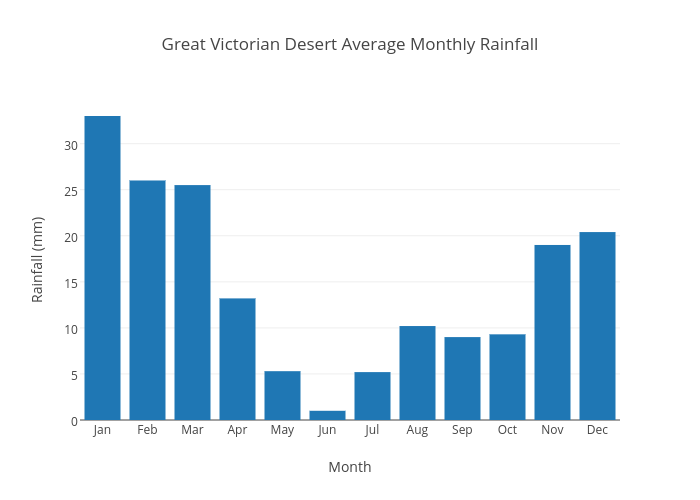
\includegraphics[scale = 0.2]{fig/pic10}
\vspace{10cm}
 
\includegraphics[scale=0.16]{fig/pic12}
\end{figure}
}
\end{frame}

\begin{frame}{Describing Experiments}
\onslide<1->{
\begin{itemize}
\item Decide which results to report\\
\tab \footnotesize Do not show the material with no interest to others
\end{itemize} 
}
\onslide<2-3>{
\begin{itemize}
\item State the existence of failure\\
\tab \footnotesize If a test fails on some data sets and succeeds on others, it is unethical to hide the failures
\end{itemize} 
}
\onslide<3>{
\begin{itemize}
\item Experiment relevance to the hypothesis\\
\tab \footnotesize Some experiments may lead to a dead end
\end{itemize} 
}
\end{frame}

\begin{frame}{Describing Experiments}
\onslide<1->{
\begin{itemize}
\item Describe the data\\
\tab \footnotesize How the data was gathered or created
\end{itemize} 
}

\onslide<2-3>{
\begin{itemize}
\item Notebooks\\
\tab \footnotesize Strategy used by researchers in other departments of science
\end{itemize} 
}
\onslide<3>{
\begin{itemize}
\item Online coding\\
\tab \footnotesize Strategy used in computer science keeps researchers honest
\end{itemize} 
}
\end{frame}

\begin{frame}{Discussion}
\onslide<1->{
\begin{center} Thank you for your attention!\\
 Question?
\end{center}

}
\end{frame}

\end{document}